\documentclass{standalone}
\usepackage{tikz}
\usetikzlibrary{patterns}
\usetikzlibrary{positioning}
\usetikzlibrary{patterns, positioning}
\usetikzlibrary{shapes.misc}
\usepackage[outline]{contour}
\contourlength{1.5pt} 
\usetikzlibrary{calc}
        \usepackage{relsize}
        \tikzset{fontscale/.style = {font=\relsize{#1}}}

\begin{document}
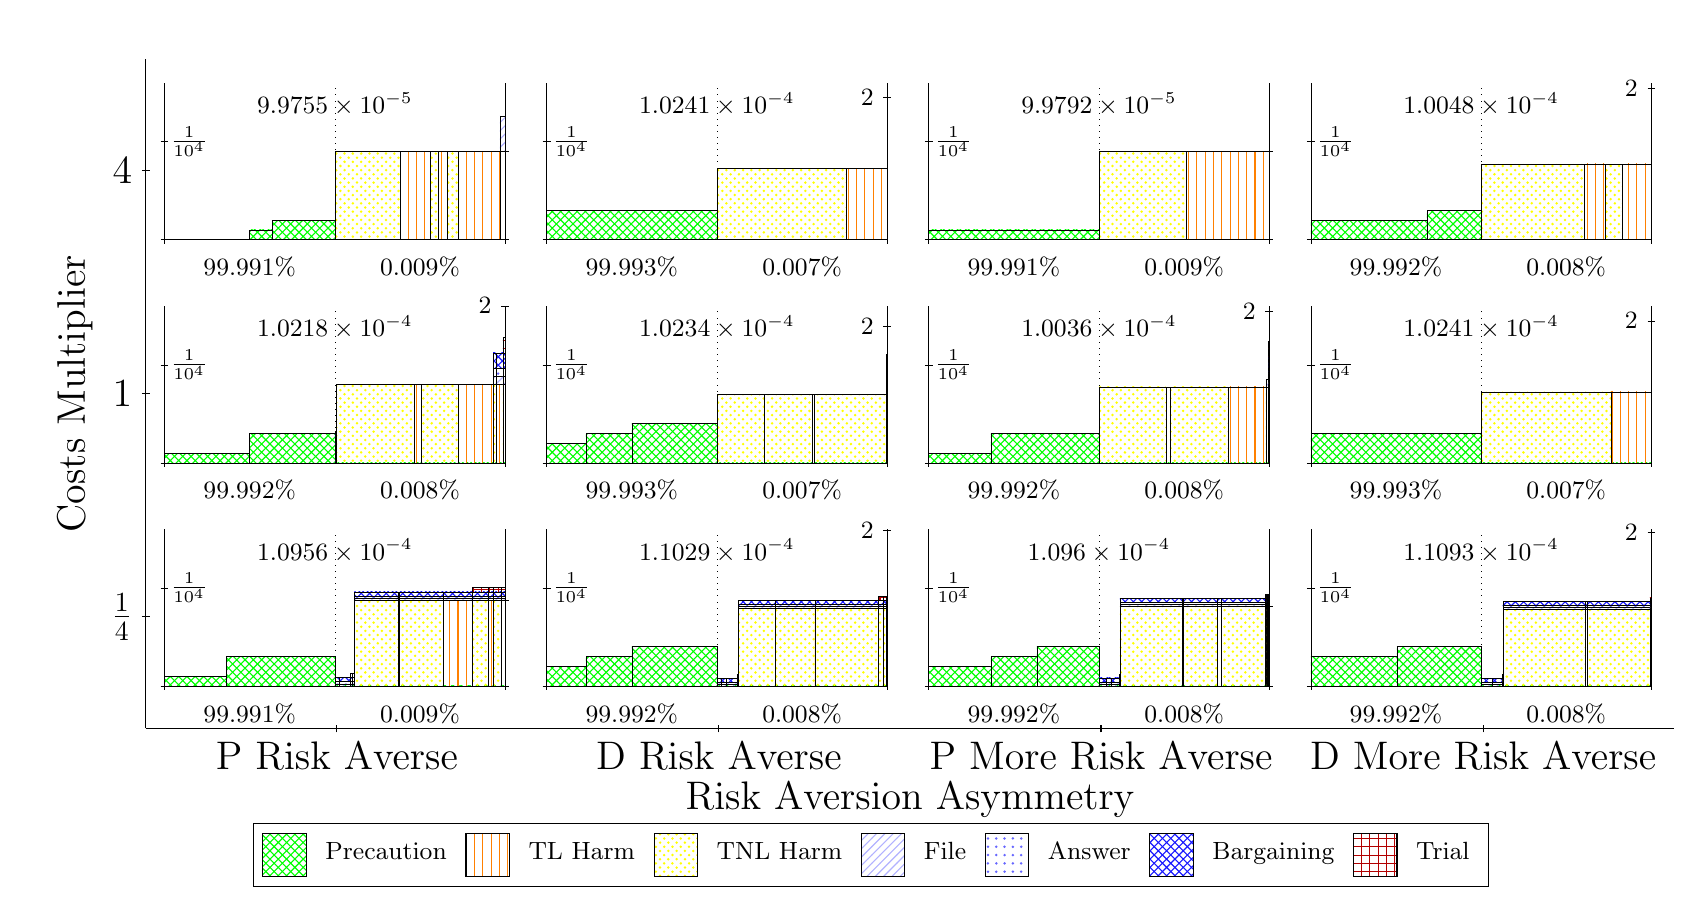
\begin{tikzpicture}
\clip(-0.5,-1.1) rectangle +(20.91,11);
\draw[black] (1,1) -- (1,9.5);
\node[rotate=90, fontscale=2, anchor=center] at (0.1, 5.25) {Costs Multiplier};
\draw[black] (0.95,2.4167) -- (1.05,2.4167);
\node[fontscale=2, anchor=east] at (0.95, 2.4167) {$\frac{1}{4}$};
\draw[black] (0.95,5.25) -- (1.05,5.25);
\node[fontscale=2, anchor=east] at (0.95, 5.25) {1};
\draw[black] (0.95,8.0833) -- (1.05,8.0833);
\node[fontscale=2, anchor=east] at (0.95, 8.0833) {4};

\draw[black] (1,1) -- (20.41,1);
\node[fontscale=2, anchor=center] at (10.705, 0.1) {Risk Aversion Asymmetry};
\draw[black] (3.4263,0.95) -- (3.4263,1.05);
\node[fontscale=2, anchor=north] at (3.4263, 0.95) {P Risk Averse};
\draw[black] (8.2788,0.95) -- (8.2788,1.05);
\node[fontscale=2, anchor=north] at (8.2788, 0.95) {D Risk Averse};
\draw[black] (13.131,0.95) -- (13.131,1.05);
\node[fontscale=2, anchor=north] at (13.131, 0.95) {P More Risk Averse};
\draw[black] (17.984,0.95) -- (17.984,1.05);
\node[fontscale=2, anchor=north] at (17.984, 0.95) {D More Risk Averse};


\draw[pattern=crosshatch, pattern color=green,draw=black,very thin] (1.2381,1.54) rectangle (2.0279,1.6645);
\draw[pattern=crosshatch, pattern color=green,draw=black,very thin] (2.0279,1.54) rectangle (3.4013,1.9135);
\draw[pattern=crosshatch, pattern color=green,draw=black,very thin] (3.4013,1.54) rectangle (3.4624,1.54);
\draw[pattern=north east lines, pattern color=blue!30,draw=black,very thin] (3.4013,1.54) rectangle (3.4624,1.5672);
\draw[pattern=dots,  pattern color=blue!60,draw=black,very thin] (3.4013,1.5672) rectangle (3.4624,1.5943);
\draw[pattern=crosshatch,      pattern color=blue!90,draw=black,very thin] (3.4013,1.5943) rectangle (3.4624,1.6486);
\draw[pattern=crosshatch, pattern color=green,draw=black,very thin] (3.4624,1.54) rectangle (3.5978,1.54);
\draw[pattern=north east lines, pattern color=blue!30,draw=black,very thin] (3.4624,1.54) rectangle (3.5978,1.5672);
\draw[pattern=dots,  pattern color=blue!60,draw=black,very thin] (3.4624,1.5672) rectangle (3.5978,1.5943);
\draw[pattern=crosshatch,      pattern color=blue!90,draw=black,very thin] (3.4624,1.5943) rectangle (3.5978,1.6486);
\draw[pattern=crosshatch, pattern color=green,draw=black,very thin] (3.5978,1.54) rectangle (3.6273,1.54);
\draw[pattern=north east lines, pattern color=blue!30,draw=black,very thin] (3.5978,1.54) rectangle (3.6273,1.5672);
\draw[pattern=dots,  pattern color=blue!60,draw=black,very thin] (3.5978,1.5672) rectangle (3.6273,1.5943);
\draw[pattern=crosshatch,      pattern color=blue!90,draw=black,very thin] (3.5978,1.5943) rectangle (3.6273,1.6486);
\draw[pattern=grid,            pattern color=red!70!black,draw=black,very thin] (3.5978,1.6486) rectangle (3.6273,1.7029);
\draw[pattern=crosshatch, pattern color=green,draw=black,very thin] (3.6273,1.54) rectangle (3.6493,1.54);
\draw[pattern=north east lines, pattern color=blue!30,draw=black,very thin] (3.6273,1.54) rectangle (3.6493,1.5672);
\draw[pattern=dots,  pattern color=blue!60,draw=black,very thin] (3.6273,1.5672) rectangle (3.6493,1.5943);
\draw[pattern=crosshatch,      pattern color=blue!90,draw=black,very thin] (3.6273,1.5943) rectangle (3.6493,1.6486);
\draw[pattern=grid,            pattern color=red!70!black,draw=black,very thin] (3.6273,1.6486) rectangle (3.6493,1.7029);
\draw[pattern=crosshatch, pattern color=green,draw=black,very thin] (3.6493,1.54) rectangle (4.2081,1.54);
\draw[pattern=crosshatch dots, pattern color=yellow,draw=black,very thin] (3.6493,1.54) rectangle (4.2081,2.6257);
\draw[pattern=north east lines, pattern color=blue!30,draw=black,very thin] (3.6493,2.6257) rectangle (4.2081,2.6528);
\draw[pattern=dots,  pattern color=blue!60,draw=black,very thin] (3.6493,2.6528) rectangle (4.2081,2.68);
\draw[pattern=crosshatch,      pattern color=blue!90,draw=black,very thin] (3.6493,2.68) rectangle (4.2081,2.7342);
\draw[pattern=crosshatch, pattern color=green,draw=black,very thin] (4.2081,1.54) rectangle (4.2159,1.54);
\draw[pattern=vertical lines, pattern color=orange,draw=black,very thin] (4.2081,1.54) rectangle (4.2159,2.6257);
\draw[pattern=north east lines, pattern color=blue!30,draw=black,very thin] (4.2081,2.6257) rectangle (4.2159,2.6528);
\draw[pattern=dots,  pattern color=blue!60,draw=black,very thin] (4.2081,2.6528) rectangle (4.2159,2.68);
\draw[pattern=crosshatch,      pattern color=blue!90,draw=black,very thin] (4.2081,2.68) rectangle (4.2159,2.7342);
\draw[pattern=crosshatch, pattern color=green,draw=black,very thin] (4.2159,1.54) rectangle (4.7767,1.54);
\draw[pattern=crosshatch dots, pattern color=yellow,draw=black,very thin] (4.2159,1.54) rectangle (4.7767,2.6257);
\draw[pattern=north east lines, pattern color=blue!30,draw=black,very thin] (4.2159,2.6257) rectangle (4.7767,2.6528);
\draw[pattern=dots,  pattern color=blue!60,draw=black,very thin] (4.2159,2.6528) rectangle (4.7767,2.68);
\draw[pattern=crosshatch,      pattern color=blue!90,draw=black,very thin] (4.2159,2.68) rectangle (4.7767,2.7343);
\draw[pattern=crosshatch, pattern color=green,draw=black,very thin] (4.7767,1.54) rectangle (5.1473,1.54);
\draw[pattern=vertical lines, pattern color=orange,draw=black,very thin] (4.7767,1.54) rectangle (5.1473,2.6257);
\draw[pattern=north east lines, pattern color=blue!30,draw=black,very thin] (4.7767,2.6257) rectangle (5.1473,2.6528);
\draw[pattern=dots,  pattern color=blue!60,draw=black,very thin] (4.7767,2.6528) rectangle (5.1473,2.68);
\draw[pattern=crosshatch,      pattern color=blue!90,draw=black,very thin] (4.7767,2.68) rectangle (5.1473,2.7343);
\draw[pattern=crosshatch, pattern color=green,draw=black,very thin] (5.1473,1.54) rectangle (5.3541,1.54);
\draw[pattern=crosshatch dots, pattern color=yellow,draw=black,very thin] (5.1473,1.54) rectangle (5.3541,2.6257);
\draw[pattern=north east lines, pattern color=blue!30,draw=black,very thin] (5.1473,2.6257) rectangle (5.3541,2.6528);
\draw[pattern=dots,  pattern color=blue!60,draw=black,very thin] (5.1473,2.6528) rectangle (5.3541,2.68);
\draw[pattern=crosshatch,      pattern color=blue!90,draw=black,very thin] (5.1473,2.68) rectangle (5.3541,2.7342);
\draw[pattern=grid,            pattern color=red!70!black,draw=black,very thin] (5.1473,2.7342) rectangle (5.3541,2.7885);
\draw[pattern=crosshatch, pattern color=green,draw=black,very thin] (5.3541,1.54) rectangle (5.4147,1.54);
\draw[pattern=vertical lines, pattern color=orange,draw=black,very thin] (5.3541,1.54) rectangle (5.4147,2.6257);
\draw[pattern=north east lines, pattern color=blue!30,draw=black,very thin] (5.3541,2.6257) rectangle (5.4147,2.6528);
\draw[pattern=dots,  pattern color=blue!60,draw=black,very thin] (5.3541,2.6528) rectangle (5.4147,2.68);
\draw[pattern=crosshatch,      pattern color=blue!90,draw=black,very thin] (5.3541,2.68) rectangle (5.4147,2.7342);
\draw[pattern=grid,            pattern color=red!70!black,draw=black,very thin] (5.3541,2.7342) rectangle (5.4147,2.7885);
\draw[pattern=crosshatch, pattern color=green,draw=black,very thin] (5.4147,1.54) rectangle (5.5113,1.54);
\draw[pattern=crosshatch dots, pattern color=yellow,draw=black,very thin] (5.4147,1.54) rectangle (5.5113,2.6257);
\draw[pattern=north east lines, pattern color=blue!30,draw=black,very thin] (5.4147,2.6257) rectangle (5.5113,2.6528);
\draw[pattern=dots,  pattern color=blue!60,draw=black,very thin] (5.4147,2.6528) rectangle (5.5113,2.68);
\draw[pattern=crosshatch,      pattern color=blue!90,draw=black,very thin] (5.4147,2.68) rectangle (5.5113,2.7343);
\draw[pattern=grid,            pattern color=red!70!black,draw=black,very thin] (5.4147,2.7343) rectangle (5.5113,2.7886);
\draw[pattern=crosshatch, pattern color=green,draw=black,very thin] (5.5113,1.54) rectangle (5.5644,1.54);
\draw[pattern=vertical lines, pattern color=orange,draw=black,very thin] (5.5113,1.54) rectangle (5.5644,2.6257);
\draw[pattern=north east lines, pattern color=blue!30,draw=black,very thin] (5.5113,2.6257) rectangle (5.5644,2.6528);
\draw[pattern=dots,  pattern color=blue!60,draw=black,very thin] (5.5113,2.6528) rectangle (5.5644,2.68);
\draw[pattern=crosshatch,      pattern color=blue!90,draw=black,very thin] (5.5113,2.68) rectangle (5.5644,2.7343);
\draw[pattern=grid,            pattern color=red!70!black,draw=black,very thin] (5.5113,2.7343) rectangle (5.5644,2.7886);
\node[font=\small,text=black,anchor=north] at (3.4013, 3.5333) {$1.0956\times 10^{-4}$};
\draw[black,very thin] (1.2381,1.54) -- (1.2381,3.5333);
\draw[black,very thin] (1.1881,1.54) -- (1.2881,1.54);
\node[font=\small,text=black, anchor=west] at (1.1881, 1.54) {};
\draw[black,very thin] (1.1881,2.785) -- (1.2881,2.785);
\node[font=\small,text=black, anchor=west] at (1.1881, 2.785) {$\frac{1}{10^{4}}$};

\draw[black,dotted,very thin] (3.4013,1.5998) -- (3.4013,3.4735);
\draw[black,very thin] (5.5644,1.54) -- (5.5644,3.5333);
\draw[black,very thin] (5.5144,1.54) -- (5.6144,1.54);
\node[font=\small,text=black, anchor=east] at (5.5144, 1.54) {\contour{white}{}};
\draw[black,very thin] (5.5144,2.6257) -- (5.6144,2.6257);
\node[font=\small,text=black, anchor=east] at (5.5144, 2.6257) {\contour{white}{}};

\draw[black,very thin] (1.2381,1.54) -- (5.5644,1.54);
\draw[black,very thin] (1.2381,1.49) -- (1.2381,1.59);
\node[font=\small,text=black, anchor=north] at (1.2381, 1.49) {};
\draw[black,very thin] (5.5644,1.49) -- (5.5644,1.59);
\node[font=\small,text=black, anchor=north] at (5.5644, 1.49) {};

\node[font=\small,text=black,anchor=south] at (2.3197, 0.94) {99.991\%};
\node[font=\small,text=black,anchor=south] at (4.4828, 0.94) {0.009\%};

\draw[pattern=crosshatch, pattern color=green,draw=black,very thin] (6.0906,1.54) rectangle (6.5882,1.789);
\draw[pattern=crosshatch, pattern color=green,draw=black,very thin] (6.5882,1.54) rectangle (7.1722,1.9135);
\draw[pattern=crosshatch, pattern color=green,draw=black,very thin] (7.1722,1.54) rectangle (8.2538,2.038);
\draw[pattern=crosshatch, pattern color=green,draw=black,very thin] (8.2538,1.54) rectangle (8.3085,1.54);
\draw[pattern=north east lines, pattern color=blue!30,draw=black,very thin] (8.2538,1.54) rectangle (8.3085,1.5647);
\draw[pattern=dots,  pattern color=blue!60,draw=black,very thin] (8.2538,1.5647) rectangle (8.3085,1.5895);
\draw[pattern=crosshatch,      pattern color=blue!90,draw=black,very thin] (8.2538,1.5895) rectangle (8.3085,1.6389);
\draw[pattern=crosshatch, pattern color=green,draw=black,very thin] (8.3085,1.54) rectangle (8.3753,1.54);
\draw[pattern=north east lines, pattern color=blue!30,draw=black,very thin] (8.3085,1.54) rectangle (8.3753,1.5647);
\draw[pattern=dots,  pattern color=blue!60,draw=black,very thin] (8.3085,1.5647) rectangle (8.3753,1.5895);
\draw[pattern=crosshatch,      pattern color=blue!90,draw=black,very thin] (8.3085,1.5895) rectangle (8.3753,1.6389);
\draw[pattern=crosshatch, pattern color=green,draw=black,very thin] (8.3753,1.54) rectangle (8.5115,1.54);
\draw[pattern=north east lines, pattern color=blue!30,draw=black,very thin] (8.3753,1.54) rectangle (8.5115,1.5648);
\draw[pattern=dots,  pattern color=blue!60,draw=black,very thin] (8.3753,1.5648) rectangle (8.5115,1.5895);
\draw[pattern=crosshatch,      pattern color=blue!90,draw=black,very thin] (8.3753,1.5895) rectangle (8.5115,1.6389);
\draw[pattern=crosshatch, pattern color=green,draw=black,very thin] (8.5115,1.54) rectangle (8.5194,1.54);
\draw[pattern=north east lines, pattern color=blue!30,draw=black,very thin] (8.5115,1.54) rectangle (8.5194,1.5647);
\draw[pattern=dots,  pattern color=blue!60,draw=black,very thin] (8.5115,1.5647) rectangle (8.5194,1.5895);
\draw[pattern=crosshatch,      pattern color=blue!90,draw=black,very thin] (8.5115,1.5895) rectangle (8.5194,1.6389);
\draw[pattern=grid,            pattern color=red!70!black,draw=black,very thin] (8.5115,1.6389) rectangle (8.5194,1.6883);
\draw[pattern=crosshatch, pattern color=green,draw=black,very thin] (8.5194,1.54) rectangle (8.5261,1.54);
\draw[pattern=north east lines, pattern color=blue!30,draw=black,very thin] (8.5194,1.54) rectangle (8.5261,1.5647);
\draw[pattern=dots,  pattern color=blue!60,draw=black,very thin] (8.5194,1.5647) rectangle (8.5261,1.5895);
\draw[pattern=crosshatch,      pattern color=blue!90,draw=black,very thin] (8.5194,1.5895) rectangle (8.5261,1.6389);
\draw[pattern=grid,            pattern color=red!70!black,draw=black,very thin] (8.5194,1.6389) rectangle (8.5261,1.6883);
\draw[pattern=crosshatch, pattern color=green,draw=black,very thin] (8.5261,1.54) rectangle (8.9985,1.54);
\draw[pattern=crosshatch dots, pattern color=yellow,draw=black,very thin] (8.5261,1.54) rectangle (8.9985,2.5288);
\draw[pattern=north east lines, pattern color=blue!30,draw=black,very thin] (8.5261,2.5288) rectangle (8.9985,2.5535);
\draw[pattern=dots,  pattern color=blue!60,draw=black,very thin] (8.5261,2.5535) rectangle (8.9985,2.5782);
\draw[pattern=crosshatch,      pattern color=blue!90,draw=black,very thin] (8.5261,2.5782) rectangle (8.9985,2.6276);
\draw[pattern=crosshatch, pattern color=green,draw=black,very thin] (8.9985,1.54) rectangle (8.9991,1.54);
\draw[pattern=vertical lines, pattern color=orange,draw=black,very thin] (8.9985,1.54) rectangle (8.9991,2.5288);
\draw[pattern=north east lines, pattern color=blue!30,draw=black,very thin] (8.9985,2.5288) rectangle (8.9991,2.5535);
\draw[pattern=dots,  pattern color=blue!60,draw=black,very thin] (8.9985,2.5535) rectangle (8.9991,2.5782);
\draw[pattern=crosshatch,      pattern color=blue!90,draw=black,very thin] (8.9985,2.5782) rectangle (8.9991,2.6276);
\draw[pattern=crosshatch, pattern color=green,draw=black,very thin] (8.9991,1.54) rectangle (9.4989,1.54);
\draw[pattern=crosshatch dots, pattern color=yellow,draw=black,very thin] (8.9991,1.54) rectangle (9.4989,2.5288);
\draw[pattern=north east lines, pattern color=blue!30,draw=black,very thin] (8.9991,2.5288) rectangle (9.4989,2.5535);
\draw[pattern=dots,  pattern color=blue!60,draw=black,very thin] (8.9991,2.5535) rectangle (9.4989,2.5782);
\draw[pattern=crosshatch,      pattern color=blue!90,draw=black,very thin] (8.9991,2.5782) rectangle (9.4989,2.6276);
\draw[pattern=crosshatch, pattern color=green,draw=black,very thin] (9.4989,1.54) rectangle (9.5073,1.54);
\draw[pattern=vertical lines, pattern color=orange,draw=black,very thin] (9.4989,1.54) rectangle (9.5073,2.5288);
\draw[pattern=north east lines, pattern color=blue!30,draw=black,very thin] (9.4989,2.5288) rectangle (9.5073,2.5535);
\draw[pattern=dots,  pattern color=blue!60,draw=black,very thin] (9.4989,2.5535) rectangle (9.5073,2.5782);
\draw[pattern=crosshatch,      pattern color=blue!90,draw=black,very thin] (9.4989,2.5782) rectangle (9.5073,2.6276);
\draw[pattern=crosshatch, pattern color=green,draw=black,very thin] (9.5073,1.54) rectangle (10.306,1.54);
\draw[pattern=crosshatch dots, pattern color=yellow,draw=black,very thin] (9.5073,1.54) rectangle (10.306,2.5288);
\draw[pattern=north east lines, pattern color=blue!30,draw=black,very thin] (9.5073,2.5288) rectangle (10.306,2.5535);
\draw[pattern=dots,  pattern color=blue!60,draw=black,very thin] (9.5073,2.5535) rectangle (10.306,2.5782);
\draw[pattern=crosshatch,      pattern color=blue!90,draw=black,very thin] (9.5073,2.5782) rectangle (10.306,2.6277);
\draw[pattern=crosshatch, pattern color=green,draw=black,very thin] (10.306,1.54) rectangle (10.367,1.54);
\draw[pattern=crosshatch dots, pattern color=yellow,draw=black,very thin] (10.306,1.54) rectangle (10.367,2.5288);
\draw[pattern=north east lines, pattern color=blue!30,draw=black,very thin] (10.306,2.5288) rectangle (10.367,2.5535);
\draw[pattern=dots,  pattern color=blue!60,draw=black,very thin] (10.306,2.5535) rectangle (10.367,2.5782);
\draw[pattern=crosshatch,      pattern color=blue!90,draw=black,very thin] (10.306,2.5782) rectangle (10.367,2.6276);
\draw[pattern=grid,            pattern color=red!70!black,draw=black,very thin] (10.306,2.6276) rectangle (10.367,2.6771);
\draw[pattern=crosshatch, pattern color=green,draw=black,very thin] (10.367,1.54) rectangle (10.371,1.54);
\draw[pattern=vertical lines, pattern color=orange,draw=black,very thin] (10.367,1.54) rectangle (10.371,2.5288);
\draw[pattern=north east lines, pattern color=blue!30,draw=black,very thin] (10.367,2.5288) rectangle (10.371,2.5535);
\draw[pattern=dots,  pattern color=blue!60,draw=black,very thin] (10.367,2.5535) rectangle (10.371,2.5782);
\draw[pattern=crosshatch,      pattern color=blue!90,draw=black,very thin] (10.367,2.5782) rectangle (10.371,2.6276);
\draw[pattern=grid,            pattern color=red!70!black,draw=black,very thin] (10.367,2.6276) rectangle (10.371,2.6771);
\draw[pattern=crosshatch, pattern color=green,draw=black,very thin] (10.371,1.54) rectangle (10.403,1.54);
\draw[pattern=crosshatch dots, pattern color=yellow,draw=black,very thin] (10.371,1.54) rectangle (10.403,2.5288);
\draw[pattern=north east lines, pattern color=blue!30,draw=black,very thin] (10.371,2.5288) rectangle (10.403,2.5535);
\draw[pattern=dots,  pattern color=blue!60,draw=black,very thin] (10.371,2.5535) rectangle (10.403,2.5782);
\draw[pattern=crosshatch,      pattern color=blue!90,draw=black,very thin] (10.371,2.5782) rectangle (10.403,2.6276);
\draw[pattern=grid,            pattern color=red!70!black,draw=black,very thin] (10.371,2.6276) rectangle (10.403,2.6771);
\draw[pattern=crosshatch, pattern color=green,draw=black,very thin] (10.403,1.54) rectangle (10.417,1.54);
\draw[pattern=vertical lines, pattern color=orange,draw=black,very thin] (10.403,1.54) rectangle (10.417,2.5288);
\draw[pattern=north east lines, pattern color=blue!30,draw=black,very thin] (10.403,2.5288) rectangle (10.417,2.5535);
\draw[pattern=dots,  pattern color=blue!60,draw=black,very thin] (10.403,2.5535) rectangle (10.417,2.5782);
\draw[pattern=crosshatch,      pattern color=blue!90,draw=black,very thin] (10.403,2.5782) rectangle (10.417,2.6276);
\draw[pattern=grid,            pattern color=red!70!black,draw=black,very thin] (10.403,2.6276) rectangle (10.417,2.6771);
\node[font=\small,text=black,anchor=north] at (8.2538, 3.5333) {$1.1029\times 10^{-4}$};
\draw[black,very thin] (6.0906,1.54) -- (6.0906,3.5333);
\draw[black,very thin] (6.0406,1.54) -- (6.1406,1.54);
\node[font=\small,text=black, anchor=west] at (6.0406, 1.54) {};
\draw[black,very thin] (6.0406,2.785) -- (6.1406,2.785);
\node[font=\small,text=black, anchor=west] at (6.0406, 2.785) {$\frac{1}{10^{4}}$};

\draw[black,dotted,very thin] (8.2538,1.5998) -- (8.2538,3.4735);
\draw[black,very thin] (10.417,1.54) -- (10.417,3.5333);
\draw[black,very thin] (10.367,3.5175) -- (10.467,3.5175);
\node[font=\small,text=black, anchor=east] at (10.367, 3.5175) {\contour{white}{2}};

\draw[black,very thin] (6.0906,1.54) -- (10.417,1.54);
\draw[black,very thin] (6.0906,1.49) -- (6.0906,1.59);
\node[font=\small,text=black, anchor=north] at (6.0906, 1.49) {};
\draw[black,very thin] (10.417,1.49) -- (10.417,1.59);
\node[font=\small,text=black, anchor=north] at (10.417, 1.49) {};

\node[font=\small,text=black,anchor=south] at (7.1722, 0.94) {99.992\%};
\node[font=\small,text=black,anchor=south] at (9.3353, 0.94) {0.008\%};

\draw[pattern=crosshatch, pattern color=green,draw=black,very thin] (10.943,1.54) rectangle (11.733,1.789);
\draw[pattern=crosshatch, pattern color=green,draw=black,very thin] (11.733,1.54) rectangle (12.316,1.9135);
\draw[pattern=crosshatch, pattern color=green,draw=black,very thin] (12.316,1.54) rectangle (13.106,2.038);
\draw[pattern=crosshatch, pattern color=green,draw=black,very thin] (13.106,1.54) rectangle (13.2,1.54);
\draw[pattern=north east lines, pattern color=blue!30,draw=black,very thin] (13.106,1.54) rectangle (13.2,1.5653);
\draw[pattern=dots,  pattern color=blue!60,draw=black,very thin] (13.106,1.5653) rectangle (13.2,1.5907);
\draw[pattern=crosshatch,      pattern color=blue!90,draw=black,very thin] (13.106,1.5907) rectangle (13.2,1.6413);
\draw[pattern=crosshatch, pattern color=green,draw=black,very thin] (13.2,1.54) rectangle (13.267,1.54);
\draw[pattern=north east lines, pattern color=blue!30,draw=black,very thin] (13.2,1.54) rectangle (13.267,1.5653);
\draw[pattern=dots,  pattern color=blue!60,draw=black,very thin] (13.2,1.5653) rectangle (13.267,1.5907);
\draw[pattern=crosshatch,      pattern color=blue!90,draw=black,very thin] (13.2,1.5907) rectangle (13.267,1.6413);
\draw[pattern=crosshatch, pattern color=green,draw=black,very thin] (13.267,1.54) rectangle (13.364,1.54);
\draw[pattern=north east lines, pattern color=blue!30,draw=black,very thin] (13.267,1.54) rectangle (13.364,1.5654);
\draw[pattern=dots,  pattern color=blue!60,draw=black,very thin] (13.267,1.5654) rectangle (13.364,1.5907);
\draw[pattern=crosshatch,      pattern color=blue!90,draw=black,very thin] (13.267,1.5907) rectangle (13.364,1.6413);
\draw[pattern=crosshatch, pattern color=green,draw=black,very thin] (13.364,1.54) rectangle (13.368,1.54);
\draw[pattern=north east lines, pattern color=blue!30,draw=black,very thin] (13.364,1.54) rectangle (13.368,1.5653);
\draw[pattern=dots,  pattern color=blue!60,draw=black,very thin] (13.364,1.5653) rectangle (13.368,1.5907);
\draw[pattern=crosshatch,      pattern color=blue!90,draw=black,very thin] (13.364,1.5907) rectangle (13.368,1.6413);
\draw[pattern=grid,            pattern color=red!70!black,draw=black,very thin] (13.364,1.6413) rectangle (13.368,1.6919);
\draw[pattern=crosshatch, pattern color=green,draw=black,very thin] (13.368,1.54) rectangle (13.372,1.54);
\draw[pattern=north east lines, pattern color=blue!30,draw=black,very thin] (13.368,1.54) rectangle (13.372,1.5653);
\draw[pattern=dots,  pattern color=blue!60,draw=black,very thin] (13.368,1.5653) rectangle (13.372,1.5907);
\draw[pattern=crosshatch,      pattern color=blue!90,draw=black,very thin] (13.368,1.5907) rectangle (13.372,1.6413);
\draw[pattern=grid,            pattern color=red!70!black,draw=black,very thin] (13.368,1.6413) rectangle (13.372,1.6919);
\draw[pattern=crosshatch, pattern color=green,draw=black,very thin] (13.372,1.54) rectangle (14.161,1.54);
\draw[pattern=crosshatch dots, pattern color=yellow,draw=black,very thin] (13.372,1.54) rectangle (14.161,2.5528);
\draw[pattern=north east lines, pattern color=blue!30,draw=black,very thin] (13.372,2.5528) rectangle (14.161,2.5781);
\draw[pattern=dots,  pattern color=blue!60,draw=black,very thin] (13.372,2.5781) rectangle (14.161,2.6034);
\draw[pattern=crosshatch,      pattern color=blue!90,draw=black,very thin] (13.372,2.6034) rectangle (14.161,2.6541);
\draw[pattern=crosshatch, pattern color=green,draw=black,very thin] (14.161,1.54) rectangle (14.173,1.54);
\draw[pattern=vertical lines, pattern color=orange,draw=black,very thin] (14.161,1.54) rectangle (14.173,2.5528);
\draw[pattern=north east lines, pattern color=blue!30,draw=black,very thin] (14.161,2.5528) rectangle (14.173,2.5781);
\draw[pattern=dots,  pattern color=blue!60,draw=black,very thin] (14.161,2.5781) rectangle (14.173,2.6034);
\draw[pattern=crosshatch,      pattern color=blue!90,draw=black,very thin] (14.161,2.6034) rectangle (14.173,2.6541);
\draw[pattern=crosshatch, pattern color=green,draw=black,very thin] (14.173,1.54) rectangle (14.603,1.54);
\draw[pattern=crosshatch dots, pattern color=yellow,draw=black,very thin] (14.173,1.54) rectangle (14.603,2.5528);
\draw[pattern=north east lines, pattern color=blue!30,draw=black,very thin] (14.173,2.5528) rectangle (14.603,2.5781);
\draw[pattern=dots,  pattern color=blue!60,draw=black,very thin] (14.173,2.5781) rectangle (14.603,2.6034);
\draw[pattern=crosshatch,      pattern color=blue!90,draw=black,very thin] (14.173,2.6034) rectangle (14.603,2.6541);
\draw[pattern=crosshatch, pattern color=green,draw=black,very thin] (14.603,1.54) rectangle (14.66,1.54);
\draw[pattern=vertical lines, pattern color=orange,draw=black,very thin] (14.603,1.54) rectangle (14.66,2.5528);
\draw[pattern=north east lines, pattern color=blue!30,draw=black,very thin] (14.603,2.5528) rectangle (14.66,2.5781);
\draw[pattern=dots,  pattern color=blue!60,draw=black,very thin] (14.603,2.5781) rectangle (14.66,2.6034);
\draw[pattern=crosshatch,      pattern color=blue!90,draw=black,very thin] (14.603,2.6034) rectangle (14.66,2.6541);
\draw[pattern=crosshatch, pattern color=green,draw=black,very thin] (14.66,1.54) rectangle (15.214,1.54);
\draw[pattern=crosshatch dots, pattern color=yellow,draw=black,very thin] (14.66,1.54) rectangle (15.214,2.5528);
\draw[pattern=north east lines, pattern color=blue!30,draw=black,very thin] (14.66,2.5528) rectangle (15.214,2.5781);
\draw[pattern=dots,  pattern color=blue!60,draw=black,very thin] (14.66,2.5781) rectangle (15.214,2.6034);
\draw[pattern=crosshatch,      pattern color=blue!90,draw=black,very thin] (14.66,2.6034) rectangle (15.214,2.6541);
\draw[pattern=crosshatch, pattern color=green,draw=black,very thin] (15.214,1.54) rectangle (15.23,1.54);
\draw[pattern=crosshatch dots, pattern color=yellow,draw=black,very thin] (15.214,1.54) rectangle (15.23,2.5528);
\draw[pattern=north east lines, pattern color=blue!30,draw=black,very thin] (15.214,2.5528) rectangle (15.23,2.5781);
\draw[pattern=dots,  pattern color=blue!60,draw=black,very thin] (15.214,2.5781) rectangle (15.23,2.6034);
\draw[pattern=crosshatch,      pattern color=blue!90,draw=black,very thin] (15.214,2.6034) rectangle (15.23,2.6541);
\draw[pattern=grid,            pattern color=red!70!black,draw=black,very thin] (15.214,2.6541) rectangle (15.23,2.7047);
\draw[pattern=crosshatch, pattern color=green,draw=black,very thin] (15.23,1.54) rectangle (15.239,1.54);
\draw[pattern=vertical lines, pattern color=orange,draw=black,very thin] (15.23,1.54) rectangle (15.239,2.5528);
\draw[pattern=north east lines, pattern color=blue!30,draw=black,very thin] (15.23,2.5528) rectangle (15.239,2.5781);
\draw[pattern=dots,  pattern color=blue!60,draw=black,very thin] (15.23,2.5781) rectangle (15.239,2.6034);
\draw[pattern=crosshatch,      pattern color=blue!90,draw=black,very thin] (15.23,2.6034) rectangle (15.239,2.6541);
\draw[pattern=grid,            pattern color=red!70!black,draw=black,very thin] (15.23,2.6541) rectangle (15.239,2.7047);
\draw[pattern=crosshatch, pattern color=green,draw=black,very thin] (15.239,1.54) rectangle (15.259,1.54);
\draw[pattern=crosshatch dots, pattern color=yellow,draw=black,very thin] (15.239,1.54) rectangle (15.259,2.5528);
\draw[pattern=north east lines, pattern color=blue!30,draw=black,very thin] (15.239,2.5528) rectangle (15.259,2.5781);
\draw[pattern=dots,  pattern color=blue!60,draw=black,very thin] (15.239,2.5781) rectangle (15.259,2.6034);
\draw[pattern=crosshatch,      pattern color=blue!90,draw=black,very thin] (15.239,2.6034) rectangle (15.259,2.6541);
\draw[pattern=grid,            pattern color=red!70!black,draw=black,very thin] (15.239,2.6541) rectangle (15.259,2.7047);
\draw[pattern=crosshatch, pattern color=green,draw=black,very thin] (15.259,1.54) rectangle (15.269,1.54);
\draw[pattern=vertical lines, pattern color=orange,draw=black,very thin] (15.259,1.54) rectangle (15.269,2.5528);
\draw[pattern=north east lines, pattern color=blue!30,draw=black,very thin] (15.259,2.5528) rectangle (15.269,2.5781);
\draw[pattern=dots,  pattern color=blue!60,draw=black,very thin] (15.259,2.5781) rectangle (15.269,2.6034);
\draw[pattern=crosshatch,      pattern color=blue!90,draw=black,very thin] (15.259,2.6034) rectangle (15.269,2.6541);
\draw[pattern=grid,            pattern color=red!70!black,draw=black,very thin] (15.259,2.6541) rectangle (15.269,2.7047);
\node[font=\small,text=black,anchor=north] at (13.106, 3.5333) {$1.096\times 10^{-4}$};
\draw[black,very thin] (10.943,1.54) -- (10.943,3.5333);
\draw[black,very thin] (10.893,1.54) -- (10.993,1.54);
\node[font=\small,text=black, anchor=west] at (10.893, 1.54) {};
\draw[black,very thin] (10.893,2.785) -- (10.993,2.785);
\node[font=\small,text=black, anchor=west] at (10.893, 2.785) {$\frac{1}{10^{4}}$};

\draw[black,dotted,very thin] (13.106,1.5998) -- (13.106,3.4735);
\draw[black,very thin] (15.269,1.54) -- (15.269,3.5333);
\draw[black,very thin] (15.219,1.54) -- (15.319,1.54);
\node[font=\small,text=black, anchor=east] at (15.219, 1.54) {\contour{white}{}};
\draw[black,very thin] (15.219,2.5528) -- (15.319,2.5528);
\node[font=\small,text=black, anchor=east] at (15.219, 2.5528) {\contour{white}{}};

\draw[black,very thin] (10.943,1.54) -- (15.269,1.54);
\draw[black,very thin] (10.943,1.49) -- (10.943,1.59);
\node[font=\small,text=black, anchor=north] at (10.943, 1.49) {};
\draw[black,very thin] (15.269,1.49) -- (15.269,1.59);
\node[font=\small,text=black, anchor=north] at (15.269, 1.49) {};

\node[font=\small,text=black,anchor=south] at (12.025, 0.94) {99.992\%};
\node[font=\small,text=black,anchor=south] at (14.188, 0.94) {0.008\%};

\draw[pattern=crosshatch, pattern color=green,draw=black,very thin] (15.796,1.54) rectangle (16.89,1.9135);
\draw[pattern=crosshatch, pattern color=green,draw=black,very thin] (16.89,1.54) rectangle (17.959,2.038);
\draw[pattern=crosshatch, pattern color=green,draw=black,very thin] (17.959,1.54) rectangle (18.096,1.54);
\draw[pattern=north east lines, pattern color=blue!30,draw=black,very thin] (17.959,1.54) rectangle (18.096,1.5644);
\draw[pattern=dots,  pattern color=blue!60,draw=black,very thin] (17.959,1.5644) rectangle (18.096,1.5887);
\draw[pattern=crosshatch,      pattern color=blue!90,draw=black,very thin] (17.959,1.5887) rectangle (18.096,1.6373);
\draw[pattern=crosshatch, pattern color=green,draw=black,very thin] (18.096,1.54) rectangle (18.233,1.54);
\draw[pattern=north east lines, pattern color=blue!30,draw=black,very thin] (18.096,1.54) rectangle (18.233,1.5644);
\draw[pattern=dots,  pattern color=blue!60,draw=black,very thin] (18.096,1.5644) rectangle (18.233,1.5887);
\draw[pattern=crosshatch,      pattern color=blue!90,draw=black,very thin] (18.096,1.5887) rectangle (18.233,1.6373);
\draw[pattern=crosshatch, pattern color=green,draw=black,very thin] (18.233,1.54) rectangle (18.236,1.54);
\draw[pattern=north east lines, pattern color=blue!30,draw=black,very thin] (18.233,1.54) rectangle (18.236,1.5644);
\draw[pattern=dots,  pattern color=blue!60,draw=black,very thin] (18.233,1.5644) rectangle (18.236,1.5887);
\draw[pattern=crosshatch,      pattern color=blue!90,draw=black,very thin] (18.233,1.5887) rectangle (18.236,1.6373);
\draw[pattern=grid,            pattern color=red!70!black,draw=black,very thin] (18.233,1.6373) rectangle (18.236,1.686);
\draw[pattern=crosshatch, pattern color=green,draw=black,very thin] (18.236,1.54) rectangle (19.284,1.54);
\draw[pattern=crosshatch dots, pattern color=yellow,draw=black,very thin] (18.236,1.54) rectangle (19.284,2.5129);
\draw[pattern=north east lines, pattern color=blue!30,draw=black,very thin] (18.236,2.5129) rectangle (19.284,2.5372);
\draw[pattern=dots,  pattern color=blue!60,draw=black,very thin] (18.236,2.5372) rectangle (19.284,2.5615);
\draw[pattern=crosshatch,      pattern color=blue!90,draw=black,very thin] (18.236,2.5615) rectangle (19.284,2.6102);
\draw[pattern=crosshatch, pattern color=green,draw=black,very thin] (19.284,1.54) rectangle (19.302,1.54);
\draw[pattern=vertical lines, pattern color=orange,draw=black,very thin] (19.284,1.54) rectangle (19.302,2.5129);
\draw[pattern=north east lines, pattern color=blue!30,draw=black,very thin] (19.284,2.5129) rectangle (19.302,2.5372);
\draw[pattern=dots,  pattern color=blue!60,draw=black,very thin] (19.284,2.5372) rectangle (19.302,2.5615);
\draw[pattern=crosshatch,      pattern color=blue!90,draw=black,very thin] (19.284,2.5615) rectangle (19.302,2.6102);
\draw[pattern=crosshatch, pattern color=green,draw=black,very thin] (19.302,1.54) rectangle (20.103,1.54);
\draw[pattern=crosshatch dots, pattern color=yellow,draw=black,very thin] (19.302,1.54) rectangle (20.103,2.5129);
\draw[pattern=north east lines, pattern color=blue!30,draw=black,very thin] (19.302,2.5129) rectangle (20.103,2.5372);
\draw[pattern=dots,  pattern color=blue!60,draw=black,very thin] (19.302,2.5372) rectangle (20.103,2.5615);
\draw[pattern=crosshatch,      pattern color=blue!90,draw=black,very thin] (19.302,2.5615) rectangle (20.103,2.6102);
\draw[pattern=crosshatch, pattern color=green,draw=black,very thin] (20.103,1.54) rectangle (20.114,1.54);
\draw[pattern=crosshatch dots, pattern color=yellow,draw=black,very thin] (20.103,1.54) rectangle (20.114,2.5129);
\draw[pattern=north east lines, pattern color=blue!30,draw=black,very thin] (20.103,2.5129) rectangle (20.114,2.5372);
\draw[pattern=dots,  pattern color=blue!60,draw=black,very thin] (20.103,2.5372) rectangle (20.114,2.5615);
\draw[pattern=crosshatch,      pattern color=blue!90,draw=black,very thin] (20.103,2.5615) rectangle (20.114,2.6102);
\draw[pattern=grid,            pattern color=red!70!black,draw=black,very thin] (20.103,2.6102) rectangle (20.114,2.6588);
\draw[pattern=crosshatch, pattern color=green,draw=black,very thin] (20.114,1.54) rectangle (20.122,1.54);
\draw[pattern=vertical lines, pattern color=orange,draw=black,very thin] (20.114,1.54) rectangle (20.122,2.5129);
\draw[pattern=north east lines, pattern color=blue!30,draw=black,very thin] (20.114,2.5129) rectangle (20.122,2.5372);
\draw[pattern=dots,  pattern color=blue!60,draw=black,very thin] (20.114,2.5372) rectangle (20.122,2.5615);
\draw[pattern=crosshatch,      pattern color=blue!90,draw=black,very thin] (20.114,2.5615) rectangle (20.122,2.6102);
\draw[pattern=grid,            pattern color=red!70!black,draw=black,very thin] (20.114,2.6102) rectangle (20.122,2.6588);
\node[font=\small,text=black,anchor=north] at (17.959, 3.5333) {$1.1093\times 10^{-4}$};
\draw[black,very thin] (15.796,1.54) -- (15.796,3.5333);
\draw[black,very thin] (15.746,1.54) -- (15.846,1.54);
\node[font=\small,text=black, anchor=west] at (15.746, 1.54) {};
\draw[black,very thin] (15.746,2.785) -- (15.846,2.785);
\node[font=\small,text=black, anchor=west] at (15.746, 2.785) {$\frac{1}{10^{4}}$};

\draw[black,dotted,very thin] (17.959,1.5998) -- (17.959,3.4735);
\draw[black,very thin] (20.122,1.54) -- (20.122,3.5333);
\draw[black,very thin] (20.072,3.4857) -- (20.172,3.4857);
\node[font=\small,text=black, anchor=east] at (20.072, 3.4857) {\contour{white}{2}};

\draw[black,very thin] (15.796,1.54) -- (20.122,1.54);
\draw[black,very thin] (15.796,1.49) -- (15.796,1.59);
\node[font=\small,text=black, anchor=north] at (15.796, 1.49) {};
\draw[black,very thin] (20.122,1.49) -- (20.122,1.59);
\node[font=\small,text=black, anchor=north] at (20.122, 1.49) {};

\node[font=\small,text=black,anchor=south] at (16.877, 0.94) {99.992\%};
\node[font=\small,text=black,anchor=south] at (19.04, 0.94) {0.008\%};

\draw[pattern=crosshatch, pattern color=green,draw=black,very thin] (1.2381,4.3733) rectangle (2.3197,4.4978);
\draw[pattern=crosshatch, pattern color=green,draw=black,very thin] (2.3197,4.3733) rectangle (3.4013,4.7468);
\draw[pattern=crosshatch, pattern color=green,draw=black,very thin] (3.4013,4.3733) rectangle (3.415,4.3733);
\draw[pattern=north east lines, pattern color=blue!30,draw=black,very thin] (3.4013,4.3733) rectangle (3.415,4.473);
\draw[pattern=dots,  pattern color=blue!60,draw=black,very thin] (3.4013,4.473) rectangle (3.415,4.5727);
\draw[pattern=crosshatch,      pattern color=blue!90,draw=black,very thin] (3.4013,4.5727) rectangle (3.415,4.772);
\draw[pattern=crosshatch, pattern color=green,draw=black,very thin] (3.415,4.3733) rectangle (3.4184,4.3733);
\draw[pattern=north east lines, pattern color=blue!30,draw=black,very thin] (3.415,4.3733) rectangle (3.4184,4.473);
\draw[pattern=dots,  pattern color=blue!60,draw=black,very thin] (3.415,4.473) rectangle (3.4184,4.5727);
\draw[pattern=crosshatch,      pattern color=blue!90,draw=black,very thin] (3.415,4.5727) rectangle (3.4184,4.772);
\draw[pattern=grid,            pattern color=red!70!black,draw=black,very thin] (3.415,4.772) rectangle (3.4184,4.9713);
\draw[pattern=crosshatch, pattern color=green,draw=black,very thin] (3.4184,4.3733) rectangle (4.4077,4.3733);
\draw[pattern=crosshatch dots, pattern color=yellow,draw=black,very thin] (3.4184,4.3733) rectangle (4.4077,5.37);
\draw[pattern=crosshatch, pattern color=green,draw=black,very thin] (4.4077,4.3733) rectangle (4.503,4.3733);
\draw[pattern=vertical lines, pattern color=orange,draw=black,very thin] (4.4077,4.3733) rectangle (4.503,5.37);
\draw[pattern=crosshatch, pattern color=green,draw=black,very thin] (4.503,4.3733) rectangle (4.9676,4.3734);
\draw[pattern=crosshatch dots, pattern color=yellow,draw=black,very thin] (4.503,4.3734) rectangle (4.9676,5.37);
\draw[pattern=crosshatch, pattern color=green,draw=black,very thin] (4.9676,4.3733) rectangle (5.4116,4.3734);
\draw[pattern=vertical lines, pattern color=orange,draw=black,very thin] (4.9676,4.3734) rectangle (5.4116,5.37);
\draw[pattern=crosshatch, pattern color=green,draw=black,very thin] (5.4116,4.3733) rectangle (5.4555,4.3733);
\draw[pattern=crosshatch dots, pattern color=yellow,draw=black,very thin] (5.4116,4.3733) rectangle (5.4555,5.37);
\draw[pattern=north east lines, pattern color=blue!30,draw=black,very thin] (5.4116,5.37) rectangle (5.4555,5.4697);
\draw[pattern=dots,  pattern color=blue!60,draw=black,very thin] (5.4116,5.4697) rectangle (5.4555,5.5693);
\draw[pattern=crosshatch,      pattern color=blue!90,draw=black,very thin] (5.4116,5.5693) rectangle (5.4555,5.7687);
\draw[pattern=crosshatch, pattern color=green,draw=black,very thin] (5.4555,4.3733) rectangle (5.5338,4.3733);
\draw[pattern=vertical lines, pattern color=orange,draw=black,very thin] (5.4555,4.3733) rectangle (5.5338,5.37);
\draw[pattern=north east lines, pattern color=blue!30,draw=black,very thin] (5.4555,5.37) rectangle (5.5338,5.4697);
\draw[pattern=dots,  pattern color=blue!60,draw=black,very thin] (5.4555,5.4697) rectangle (5.5338,5.5693);
\draw[pattern=crosshatch,      pattern color=blue!90,draw=black,very thin] (5.4555,5.5693) rectangle (5.5338,5.7687);
\draw[pattern=crosshatch, pattern color=green,draw=black,very thin] (5.5338,4.3733) rectangle (5.5428,4.3733);
\draw[pattern=crosshatch dots, pattern color=yellow,draw=black,very thin] (5.5338,4.3733) rectangle (5.5428,5.37);
\draw[pattern=north east lines, pattern color=blue!30,draw=black,very thin] (5.5338,5.37) rectangle (5.5428,5.4697);
\draw[pattern=dots,  pattern color=blue!60,draw=black,very thin] (5.5338,5.4697) rectangle (5.5428,5.5693);
\draw[pattern=crosshatch,      pattern color=blue!90,draw=black,very thin] (5.5338,5.5693) rectangle (5.5428,5.7687);
\draw[pattern=grid,            pattern color=red!70!black,draw=black,very thin] (5.5338,5.7687) rectangle (5.5428,5.968);
\draw[pattern=crosshatch, pattern color=green,draw=black,very thin] (5.5428,4.3733) rectangle (5.5644,4.3733);
\draw[pattern=vertical lines, pattern color=orange,draw=black,very thin] (5.5428,4.3733) rectangle (5.5644,5.37);
\draw[pattern=north east lines, pattern color=blue!30,draw=black,very thin] (5.5428,5.37) rectangle (5.5644,5.4697);
\draw[pattern=dots,  pattern color=blue!60,draw=black,very thin] (5.5428,5.4697) rectangle (5.5644,5.5693);
\draw[pattern=crosshatch,      pattern color=blue!90,draw=black,very thin] (5.5428,5.5693) rectangle (5.5644,5.7687);
\draw[pattern=grid,            pattern color=red!70!black,draw=black,very thin] (5.5428,5.7687) rectangle (5.5644,5.968);
\node[font=\small,text=black,anchor=north] at (3.4013, 6.3667) {$1.0218\times 10^{-4}$};
\draw[black,very thin] (1.2381,4.3733) -- (1.2381,6.3667);
\draw[black,very thin] (1.1881,4.3733) -- (1.2881,4.3733);
\node[font=\small,text=black, anchor=west] at (1.1881, 4.3733) {};
\draw[black,very thin] (1.1881,5.6183) -- (1.2881,5.6183);
\node[font=\small,text=black, anchor=west] at (1.1881, 5.6183) {$\frac{1}{10^{4}}$};

\draw[black,dotted,very thin] (3.4013,4.4331) -- (3.4013,6.3069);
\draw[black,very thin] (5.5644,4.3733) -- (5.5644,6.3667);
\draw[black,very thin] (5.5144,6.3667) -- (5.6144,6.3667);
\node[font=\small,text=black, anchor=east] at (5.5144, 6.3667) {\contour{white}{2}};

\draw[black,very thin] (1.2381,4.3733) -- (5.5644,4.3733);
\draw[black,very thin] (1.2381,4.3233) -- (1.2381,4.4233);
\node[font=\small,text=black, anchor=north] at (1.2381, 4.3233) {};
\draw[black,very thin] (5.5644,4.3233) -- (5.5644,4.4233);
\node[font=\small,text=black, anchor=north] at (5.5644, 4.3233) {};

\node[font=\small,text=black,anchor=south] at (2.3197, 3.7733) {99.992\%};
\node[font=\small,text=black,anchor=south] at (4.4828, 3.7733) {0.008\%};

\draw[pattern=crosshatch, pattern color=green,draw=black,very thin] (6.0906,4.3733) rectangle (6.5882,4.6223);
\draw[pattern=crosshatch, pattern color=green,draw=black,very thin] (6.5882,4.3733) rectangle (7.1722,4.7468);
\draw[pattern=crosshatch, pattern color=green,draw=black,very thin] (7.1722,4.3733) rectangle (8.2538,4.8713);
\draw[pattern=crosshatch, pattern color=green,draw=black,very thin] (8.2538,4.3733) rectangle (8.255,4.3734);
\draw[pattern=north east lines, pattern color=blue!30,draw=black,very thin] (8.2538,4.3734) rectangle (8.255,4.4598);
\draw[pattern=dots,  pattern color=blue!60,draw=black,very thin] (8.2538,4.4598) rectangle (8.255,4.5463);
\draw[pattern=crosshatch,      pattern color=blue!90,draw=black,very thin] (8.2538,4.5463) rectangle (8.255,4.7193);
\draw[pattern=grid,            pattern color=red!70!black,draw=black,very thin] (8.2538,4.7193) rectangle (8.255,4.8922);
\draw[pattern=crosshatch, pattern color=green,draw=black,very thin] (8.255,4.3733) rectangle (8.8568,4.3734);
\draw[pattern=crosshatch dots, pattern color=yellow,draw=black,very thin] (8.255,4.3734) rectangle (8.8568,5.2381);
\draw[pattern=crosshatch, pattern color=green,draw=black,very thin] (8.8568,4.3733) rectangle (8.8599,4.3734);
\draw[pattern=vertical lines, pattern color=orange,draw=black,very thin] (8.8568,4.3734) rectangle (8.8599,5.2381);
\draw[pattern=crosshatch, pattern color=green,draw=black,very thin] (8.8599,4.3733) rectangle (9.4688,4.3734);
\draw[pattern=crosshatch dots, pattern color=yellow,draw=black,very thin] (8.8599,4.3734) rectangle (9.4688,5.2381);
\draw[pattern=crosshatch, pattern color=green,draw=black,very thin] (9.4688,4.3733) rectangle (9.4938,4.3734);
\draw[pattern=vertical lines, pattern color=orange,draw=black,very thin] (9.4688,4.3734) rectangle (9.4938,5.2381);
\draw[pattern=crosshatch, pattern color=green,draw=black,very thin] (9.4938,4.3733) rectangle (10.407,4.3734);
\draw[pattern=crosshatch dots, pattern color=yellow,draw=black,very thin] (9.4938,4.3734) rectangle (10.407,5.2381);
\draw[pattern=crosshatch, pattern color=green,draw=black,very thin] (10.407,4.3733) rectangle (10.415,4.3734);
\draw[pattern=crosshatch dots, pattern color=yellow,draw=black,very thin] (10.407,4.3734) rectangle (10.415,5.2381);
\draw[pattern=north east lines, pattern color=blue!30,draw=black,very thin] (10.407,5.2381) rectangle (10.415,5.3246);
\draw[pattern=dots,  pattern color=blue!60,draw=black,very thin] (10.407,5.3246) rectangle (10.415,5.4111);
\draw[pattern=crosshatch,      pattern color=blue!90,draw=black,very thin] (10.407,5.4111) rectangle (10.415,5.584);
\draw[pattern=grid,            pattern color=red!70!black,draw=black,very thin] (10.407,5.584) rectangle (10.415,5.757);
\draw[pattern=crosshatch, pattern color=green,draw=black,very thin] (10.415,4.3733) rectangle (10.417,4.3734);
\draw[pattern=vertical lines, pattern color=orange,draw=black,very thin] (10.415,4.3734) rectangle (10.417,5.2381);
\draw[pattern=north east lines, pattern color=blue!30,draw=black,very thin] (10.415,5.2381) rectangle (10.417,5.3246);
\draw[pattern=dots,  pattern color=blue!60,draw=black,very thin] (10.415,5.3246) rectangle (10.417,5.4111);
\draw[pattern=crosshatch,      pattern color=blue!90,draw=black,very thin] (10.415,5.4111) rectangle (10.417,5.584);
\draw[pattern=grid,            pattern color=red!70!black,draw=black,very thin] (10.415,5.584) rectangle (10.417,5.757);
\node[font=\small,text=black,anchor=north] at (8.2538, 6.3667) {$1.0234\times 10^{-4}$};
\draw[black,very thin] (6.0906,4.3733) -- (6.0906,6.3667);
\draw[black,very thin] (6.0406,4.3733) -- (6.1406,4.3733);
\node[font=\small,text=black, anchor=west] at (6.0406, 4.3733) {};
\draw[black,very thin] (6.0406,5.6183) -- (6.1406,5.6183);
\node[font=\small,text=black, anchor=west] at (6.0406, 5.6183) {$\frac{1}{10^{4}}$};

\draw[black,dotted,very thin] (8.2538,4.4331) -- (8.2538,6.3069);
\draw[black,very thin] (10.417,4.3733) -- (10.417,6.3667);
\draw[black,very thin] (10.367,6.1029) -- (10.467,6.1029);
\node[font=\small,text=black, anchor=east] at (10.367, 6.1029) {\contour{white}{2}};

\draw[black,very thin] (6.0906,4.3733) -- (10.417,4.3733);
\draw[black,very thin] (6.0906,4.3233) -- (6.0906,4.4233);
\node[font=\small,text=black, anchor=north] at (6.0906, 4.3233) {};
\draw[black,very thin] (10.417,4.3233) -- (10.417,4.4233);
\node[font=\small,text=black, anchor=north] at (10.417, 4.3233) {};

\node[font=\small,text=black,anchor=south] at (7.1722, 3.7733) {99.993\%};
\node[font=\small,text=black,anchor=south] at (9.3353, 3.7733) {0.007\%};

\draw[pattern=crosshatch, pattern color=green,draw=black,very thin] (10.943,4.3733) rectangle (11.733,4.4978);
\draw[pattern=crosshatch, pattern color=green,draw=black,very thin] (11.733,4.3733) rectangle (13.106,4.7468);
\draw[pattern=crosshatch, pattern color=green,draw=black,very thin] (13.106,4.3733) rectangle (13.109,4.3733);
\draw[pattern=north east lines, pattern color=blue!30,draw=black,very thin] (13.106,4.3733) rectangle (13.109,4.4697);
\draw[pattern=crosshatch, pattern color=green,draw=black,very thin] (13.109,4.3733) rectangle (13.11,4.3733);
\draw[pattern=north east lines, pattern color=blue!30,draw=black,very thin] (13.109,4.3733) rectangle (13.11,4.4697);
\draw[pattern=dots,  pattern color=blue!60,draw=black,very thin] (13.109,4.4697) rectangle (13.11,4.566);
\draw[pattern=crosshatch,      pattern color=blue!90,draw=black,very thin] (13.109,4.566) rectangle (13.11,4.7587);
\draw[pattern=crosshatch, pattern color=green,draw=black,very thin] (13.11,4.3733) rectangle (13.111,4.3733);
\draw[pattern=north east lines, pattern color=blue!30,draw=black,very thin] (13.11,4.3733) rectangle (13.111,4.4697);
\draw[pattern=dots,  pattern color=blue!60,draw=black,very thin] (13.11,4.4697) rectangle (13.111,4.566);
\draw[pattern=crosshatch,      pattern color=blue!90,draw=black,very thin] (13.11,4.566) rectangle (13.111,4.7587);
\draw[pattern=grid,            pattern color=red!70!black,draw=black,very thin] (13.11,4.7587) rectangle (13.111,4.9514);
\draw[pattern=crosshatch, pattern color=green,draw=black,very thin] (13.111,4.3733) rectangle (13.955,4.3733);
\draw[pattern=crosshatch dots, pattern color=yellow,draw=black,very thin] (13.111,4.3733) rectangle (13.955,5.3368);
\draw[pattern=crosshatch, pattern color=green,draw=black,very thin] (13.955,4.3733) rectangle (14.006,4.3733);
\draw[pattern=vertical lines, pattern color=orange,draw=black,very thin] (13.955,4.3733) rectangle (14.006,5.3368);
\draw[pattern=crosshatch, pattern color=green,draw=black,very thin] (14.006,4.3733) rectangle (14.747,4.3734);
\draw[pattern=crosshatch dots, pattern color=yellow,draw=black,very thin] (14.006,4.3734) rectangle (14.747,5.3368);
\draw[pattern=crosshatch, pattern color=green,draw=black,very thin] (14.747,4.3733) rectangle (15.225,4.3734);
\draw[pattern=vertical lines, pattern color=orange,draw=black,very thin] (14.747,4.3734) rectangle (15.225,5.3368);
\draw[pattern=crosshatch, pattern color=green,draw=black,very thin] (15.225,4.3733) rectangle (15.234,4.3733);
\draw[pattern=crosshatch dots, pattern color=yellow,draw=black,very thin] (15.225,4.3733) rectangle (15.234,5.3368);
\draw[pattern=north east lines, pattern color=blue!30,draw=black,very thin] (15.225,5.3368) rectangle (15.234,5.4331);
\draw[pattern=crosshatch, pattern color=green,draw=black,very thin] (15.234,4.3733) rectangle (15.253,4.3733);
\draw[pattern=vertical lines, pattern color=orange,draw=black,very thin] (15.234,4.3733) rectangle (15.253,5.3368);
\draw[pattern=north east lines, pattern color=blue!30,draw=black,very thin] (15.234,5.3368) rectangle (15.253,5.4331);
\draw[pattern=crosshatch, pattern color=green,draw=black,very thin] (15.253,4.3733) rectangle (15.257,4.3733);
\draw[pattern=crosshatch dots, pattern color=yellow,draw=black,very thin] (15.253,4.3733) rectangle (15.257,5.3368);
\draw[pattern=north east lines, pattern color=blue!30,draw=black,very thin] (15.253,5.3368) rectangle (15.257,5.4331);
\draw[pattern=dots,  pattern color=blue!60,draw=black,very thin] (15.253,5.4331) rectangle (15.257,5.5294);
\draw[pattern=crosshatch,      pattern color=blue!90,draw=black,very thin] (15.253,5.5294) rectangle (15.257,5.7221);
\draw[pattern=crosshatch, pattern color=green,draw=black,very thin] (15.257,4.3733) rectangle (15.259,4.3733);
\draw[pattern=vertical lines, pattern color=orange,draw=black,very thin] (15.257,4.3733) rectangle (15.259,5.3368);
\draw[pattern=north east lines, pattern color=blue!30,draw=black,very thin] (15.257,5.3368) rectangle (15.259,5.4331);
\draw[pattern=dots,  pattern color=blue!60,draw=black,very thin] (15.257,5.4331) rectangle (15.259,5.5294);
\draw[pattern=crosshatch,      pattern color=blue!90,draw=black,very thin] (15.257,5.5294) rectangle (15.259,5.7221);
\draw[pattern=crosshatch, pattern color=green,draw=black,very thin] (15.259,4.3733) rectangle (15.264,4.3733);
\draw[pattern=crosshatch dots, pattern color=yellow,draw=black,very thin] (15.259,4.3733) rectangle (15.264,5.3368);
\draw[pattern=north east lines, pattern color=blue!30,draw=black,very thin] (15.259,5.3368) rectangle (15.264,5.4331);
\draw[pattern=dots,  pattern color=blue!60,draw=black,very thin] (15.259,5.4331) rectangle (15.264,5.5294);
\draw[pattern=crosshatch,      pattern color=blue!90,draw=black,very thin] (15.259,5.5294) rectangle (15.264,5.7221);
\draw[pattern=grid,            pattern color=red!70!black,draw=black,very thin] (15.259,5.7221) rectangle (15.264,5.9148);
\draw[pattern=crosshatch, pattern color=green,draw=black,very thin] (15.264,4.3733) rectangle (15.269,4.3733);
\draw[pattern=vertical lines, pattern color=orange,draw=black,very thin] (15.264,4.3733) rectangle (15.269,5.3368);
\draw[pattern=north east lines, pattern color=blue!30,draw=black,very thin] (15.264,5.3368) rectangle (15.269,5.4331);
\draw[pattern=dots,  pattern color=blue!60,draw=black,very thin] (15.264,5.4331) rectangle (15.269,5.5294);
\draw[pattern=crosshatch,      pattern color=blue!90,draw=black,very thin] (15.264,5.5294) rectangle (15.269,5.7221);
\draw[pattern=grid,            pattern color=red!70!black,draw=black,very thin] (15.264,5.7221) rectangle (15.269,5.9148);
\node[font=\small,text=black,anchor=north] at (13.106, 6.3667) {$1.0036\times 10^{-4}$};
\draw[black,very thin] (10.943,4.3733) -- (10.943,6.3667);
\draw[black,very thin] (10.893,4.3733) -- (10.993,4.3733);
\node[font=\small,text=black, anchor=west] at (10.893, 4.3733) {};
\draw[black,very thin] (10.893,5.6183) -- (10.993,5.6183);
\node[font=\small,text=black, anchor=west] at (10.893, 5.6183) {$\frac{1}{10^{4}}$};

\draw[black,dotted,very thin] (13.106,4.4331) -- (13.106,6.3069);
\draw[black,very thin] (15.269,4.3733) -- (15.269,6.3667);
\draw[black,very thin] (15.219,6.3002) -- (15.319,6.3002);
\node[font=\small,text=black, anchor=east] at (15.219, 6.3002) {\contour{white}{2}};

\draw[black,very thin] (10.943,4.3733) -- (15.269,4.3733);
\draw[black,very thin] (10.943,4.3233) -- (10.943,4.4233);
\node[font=\small,text=black, anchor=north] at (10.943, 4.3233) {};
\draw[black,very thin] (15.269,4.3233) -- (15.269,4.4233);
\node[font=\small,text=black, anchor=north] at (15.269, 4.3233) {};

\node[font=\small,text=black,anchor=south] at (12.025, 3.7733) {99.992\%};
\node[font=\small,text=black,anchor=south] at (14.188, 3.7733) {0.008\%};

\draw[pattern=crosshatch, pattern color=green,draw=black,very thin] (15.796,4.3733) rectangle (17.959,4.7468);
\draw[pattern=crosshatch, pattern color=green,draw=black,very thin] (17.959,4.3733) rectangle (19.606,4.3734);
\draw[pattern=crosshatch dots, pattern color=yellow,draw=black,very thin] (17.959,4.3734) rectangle (19.606,5.2749);
\draw[pattern=crosshatch, pattern color=green,draw=black,very thin] (19.606,4.3733) rectangle (20.122,4.3734);
\draw[pattern=vertical lines, pattern color=orange,draw=black,very thin] (19.606,4.3734) rectangle (20.122,5.2749);
\node[font=\small,text=black,anchor=north] at (17.959, 6.3667) {$1.0241\times 10^{-4}$};
\draw[black,very thin] (15.796,4.3733) -- (15.796,6.3667);
\draw[black,very thin] (15.746,4.3733) -- (15.846,4.3733);
\node[font=\small,text=black, anchor=west] at (15.746, 4.3733) {};
\draw[black,very thin] (15.746,5.6183) -- (15.846,5.6183);
\node[font=\small,text=black, anchor=west] at (15.746, 5.6183) {$\frac{1}{10^{4}}$};

\draw[black,dotted,very thin] (17.959,4.4331) -- (17.959,6.3069);
\draw[black,very thin] (20.122,4.3733) -- (20.122,6.3667);
\draw[black,very thin] (20.072,6.1764) -- (20.172,6.1764);
\node[font=\small,text=black, anchor=east] at (20.072, 6.1764) {\contour{white}{2}};

\draw[black,very thin] (15.796,4.3733) -- (20.122,4.3733);
\draw[black,very thin] (15.796,4.3233) -- (15.796,4.4233);
\node[font=\small,text=black, anchor=north] at (15.796, 4.3233) {};
\draw[black,very thin] (20.122,4.3233) -- (20.122,4.4233);
\node[font=\small,text=black, anchor=north] at (20.122, 4.3233) {};

\node[font=\small,text=black,anchor=south] at (16.877, 3.7733) {99.993\%};
\node[font=\small,text=black,anchor=south] at (19.04, 3.7733) {0.007\%};

\draw[pattern=crosshatch, pattern color=green,draw=black,very thin] (2.3197,7.2067) rectangle (2.6114,7.3312);
\draw[pattern=crosshatch, pattern color=green,draw=black,very thin] (2.6114,7.2067) rectangle (3.4013,7.4557);
\draw[pattern=crosshatch, pattern color=green,draw=black,very thin] (3.4013,7.2067) rectangle (3.4089,7.2067);
\draw[pattern=north east lines, pattern color=blue!30,draw=black,very thin] (3.4013,7.2067) rectangle (3.4089,7.6558);
\draw[pattern=crosshatch dots, pattern color=yellow,draw=black,very thin] (3.4089,7.2067) rectangle (4.2346,8.3294);
\draw[pattern=vertical lines, pattern color=orange,draw=black,very thin] (4.2346,7.2067) rectangle (4.6083,8.3294);
\draw[pattern=crosshatch, pattern color=green,draw=black,very thin] (4.6083,7.2067) rectangle (4.7124,7.2067);
\draw[pattern=crosshatch dots, pattern color=yellow,draw=black,very thin] (4.6083,7.2067) rectangle (4.7124,8.3294);
\draw[pattern=crosshatch, pattern color=green,draw=black,very thin] (4.7124,7.2067) rectangle (4.8297,7.2067);
\draw[pattern=vertical lines, pattern color=orange,draw=black,very thin] (4.7124,7.2067) rectangle (4.8297,8.3294);
\draw[pattern=crosshatch, pattern color=green,draw=black,very thin] (4.8297,7.2067) rectangle (4.9675,7.2067);
\draw[pattern=crosshatch dots, pattern color=yellow,draw=black,very thin] (4.8297,7.2067) rectangle (4.9675,8.3294);
\draw[pattern=crosshatch, pattern color=green,draw=black,very thin] (4.9675,7.2067) rectangle (5.4974,7.2067);
\draw[pattern=vertical lines, pattern color=orange,draw=black,very thin] (4.9675,7.2067) rectangle (5.4974,8.3294);
\draw[pattern=crosshatch, pattern color=green,draw=black,very thin] (5.4974,7.2067) rectangle (5.5004,7.2067);
\draw[pattern=crosshatch dots, pattern color=yellow,draw=black,very thin] (5.4974,7.2067) rectangle (5.5004,8.3294);
\draw[pattern=north east lines, pattern color=blue!30,draw=black,very thin] (5.4974,8.3294) rectangle (5.5004,8.7785);
\draw[pattern=crosshatch, pattern color=green,draw=black,very thin] (5.5004,7.2067) rectangle (5.5644,7.2067);
\draw[pattern=vertical lines, pattern color=orange,draw=black,very thin] (5.5004,7.2067) rectangle (5.5644,8.3294);
\draw[pattern=north east lines, pattern color=blue!30,draw=black,very thin] (5.5004,8.3294) rectangle (5.5644,8.7785);
\node[font=\small,text=black,anchor=north] at (3.4013, 9.2) {$9.9755\times 10^{-5}$};
\draw[black,very thin] (1.2381,7.2067) -- (1.2381,9.2);
\draw[black,very thin] (1.1881,7.2067) -- (1.2881,7.2067);
\node[font=\small,text=black, anchor=west] at (1.1881, 7.2067) {};
\draw[black,very thin] (1.1881,8.4516) -- (1.2881,8.4516);
\node[font=\small,text=black, anchor=west] at (1.1881, 8.4516) {$\frac{1}{10^{4}}$};

\draw[black,dotted,very thin] (3.4013,7.2665) -- (3.4013,9.1402);
\draw[black,very thin] (5.5644,7.2067) -- (5.5644,9.2);
\draw[black,very thin] (5.5144,7.2067) -- (5.6144,7.2067);
\node[font=\small,text=black, anchor=east] at (5.5144, 7.2067) {\contour{white}{}};
\draw[black,very thin] (5.5144,8.3294) -- (5.6144,8.3294);
\node[font=\small,text=black, anchor=east] at (5.5144, 8.3294) {\contour{white}{}};

\draw[black,very thin] (1.2381,7.2067) -- (5.5644,7.2067);
\draw[black,very thin] (1.2381,7.1567) -- (1.2381,7.2567);
\node[font=\small,text=black, anchor=north] at (1.2381, 7.1567) {};
\draw[black,very thin] (5.5644,7.1567) -- (5.5644,7.2567);
\node[font=\small,text=black, anchor=north] at (5.5644, 7.1567) {};

\node[font=\small,text=black,anchor=south] at (2.3197, 6.6067) {99.991\%};
\node[font=\small,text=black,anchor=south] at (4.4828, 6.6067) {0.009\%};

\draw[pattern=crosshatch, pattern color=green,draw=black,very thin] (6.0906,7.2067) rectangle (8.2538,7.5802);
\draw[pattern=crosshatch, pattern color=green,draw=black,very thin] (8.2538,7.2067) rectangle (9.9013,7.2067);
\draw[pattern=crosshatch dots, pattern color=yellow,draw=black,very thin] (8.2538,7.2067) rectangle (9.9013,8.1082);
\draw[pattern=crosshatch, pattern color=green,draw=black,very thin] (9.9013,7.2067) rectangle (10.417,7.2067);
\draw[pattern=vertical lines, pattern color=orange,draw=black,very thin] (9.9013,7.2067) rectangle (10.417,8.1082);
\node[font=\small,text=black,anchor=north] at (8.2538, 9.2) {$1.0241\times 10^{-4}$};
\draw[black,very thin] (6.0906,7.2067) -- (6.0906,9.2);
\draw[black,very thin] (6.0406,7.2067) -- (6.1406,7.2067);
\node[font=\small,text=black, anchor=west] at (6.0406, 7.2067) {};
\draw[black,very thin] (6.0406,8.4516) -- (6.1406,8.4516);
\node[font=\small,text=black, anchor=west] at (6.0406, 8.4516) {$\frac{1}{10^{4}}$};

\draw[black,dotted,very thin] (8.2538,7.2665) -- (8.2538,9.1402);
\draw[black,very thin] (10.417,7.2067) -- (10.417,9.2);
\draw[black,very thin] (10.367,9.0097) -- (10.467,9.0097);
\node[font=\small,text=black, anchor=east] at (10.367, 9.0097) {\contour{white}{2}};

\draw[black,very thin] (6.0906,7.2067) -- (10.417,7.2067);
\draw[black,very thin] (6.0906,7.1567) -- (6.0906,7.2567);
\node[font=\small,text=black, anchor=north] at (6.0906, 7.1567) {};
\draw[black,very thin] (10.417,7.1567) -- (10.417,7.2567);
\node[font=\small,text=black, anchor=north] at (10.417, 7.1567) {};

\node[font=\small,text=black,anchor=south] at (7.1722, 6.6067) {99.993\%};
\node[font=\small,text=black,anchor=south] at (9.3353, 6.6067) {0.007\%};

\draw[pattern=crosshatch, pattern color=green,draw=black,very thin] (10.943,7.2067) rectangle (13.106,7.3312);
\draw[pattern=crosshatch, pattern color=green,draw=black,very thin] (13.106,7.2067) rectangle (14.208,7.2067);
\draw[pattern=crosshatch dots, pattern color=yellow,draw=black,very thin] (13.106,7.2067) rectangle (14.208,8.3246);
\draw[pattern=crosshatch, pattern color=green,draw=black,very thin] (14.208,7.2067) rectangle (15.269,7.2067);
\draw[pattern=vertical lines, pattern color=orange,draw=black,very thin] (14.208,7.2067) rectangle (15.269,8.3246);
\node[font=\small,text=black,anchor=north] at (13.106, 9.2) {$9.9792\times 10^{-5}$};
\draw[black,very thin] (10.943,7.2067) -- (10.943,9.2);
\draw[black,very thin] (10.893,7.2067) -- (10.993,7.2067);
\node[font=\small,text=black, anchor=west] at (10.893, 7.2067) {};
\draw[black,very thin] (10.893,8.4516) -- (10.993,8.4516);
\node[font=\small,text=black, anchor=west] at (10.893, 8.4516) {$\frac{1}{10^{4}}$};

\draw[black,dotted,very thin] (13.106,7.2665) -- (13.106,9.1402);
\draw[black,very thin] (15.269,7.2067) -- (15.269,9.2);
\draw[black,very thin] (15.219,7.2067) -- (15.319,7.2067);
\node[font=\small,text=black, anchor=east] at (15.219, 7.2067) {\contour{white}{}};
\draw[black,very thin] (15.219,8.3246) -- (15.319,8.3246);
\node[font=\small,text=black, anchor=east] at (15.219, 8.3246) {\contour{white}{}};

\draw[black,very thin] (10.943,7.2067) -- (15.269,7.2067);
\draw[black,very thin] (10.943,7.1567) -- (10.943,7.2567);
\node[font=\small,text=black, anchor=north] at (10.943, 7.1567) {};
\draw[black,very thin] (15.269,7.1567) -- (15.269,7.2567);
\node[font=\small,text=black, anchor=north] at (15.269, 7.1567) {};

\node[font=\small,text=black,anchor=south] at (12.025, 6.6067) {99.991\%};
\node[font=\small,text=black,anchor=south] at (14.188, 6.6067) {0.009\%};

\draw[pattern=crosshatch, pattern color=green,draw=black,very thin] (15.796,7.2067) rectangle (17.269,7.4557);
\draw[pattern=crosshatch, pattern color=green,draw=black,very thin] (17.269,7.2067) rectangle (17.959,7.5802);
\draw[pattern=crosshatch, pattern color=green,draw=black,very thin] (17.959,7.2067) rectangle (19.274,7.2067);
\draw[pattern=crosshatch dots, pattern color=yellow,draw=black,very thin] (17.959,7.2067) rectangle (19.274,8.1691);
\draw[pattern=crosshatch, pattern color=green,draw=black,very thin] (19.274,7.2067) rectangle (19.535,7.2067);
\draw[pattern=vertical lines, pattern color=orange,draw=black,very thin] (19.274,7.2067) rectangle (19.535,8.1691);
\draw[pattern=crosshatch, pattern color=green,draw=black,very thin] (19.535,7.2067) rectangle (19.752,7.2067);
\draw[pattern=crosshatch dots, pattern color=yellow,draw=black,very thin] (19.535,7.2067) rectangle (19.752,8.1691);
\draw[pattern=crosshatch, pattern color=green,draw=black,very thin] (19.752,7.2067) rectangle (20.122,7.2067);
\draw[pattern=vertical lines, pattern color=orange,draw=black,very thin] (19.752,7.2067) rectangle (20.122,8.1691);
\node[font=\small,text=black,anchor=north] at (17.959, 9.2) {$1.0048\times 10^{-4}$};
\draw[black,very thin] (15.796,7.2067) -- (15.796,9.2);
\draw[black,very thin] (15.746,7.2067) -- (15.846,7.2067);
\node[font=\small,text=black, anchor=west] at (15.746, 7.2067) {};
\draw[black,very thin] (15.746,8.4516) -- (15.846,8.4516);
\node[font=\small,text=black, anchor=west] at (15.746, 8.4516) {$\frac{1}{10^{4}}$};

\draw[black,dotted,very thin] (17.959,7.2665) -- (17.959,9.1402);
\draw[black,very thin] (20.122,7.2067) -- (20.122,9.2);
\draw[black,very thin] (20.072,9.1314) -- (20.172,9.1314);
\node[font=\small,text=black, anchor=east] at (20.072, 9.1314) {\contour{white}{2}};

\draw[black,very thin] (15.796,7.2067) -- (20.122,7.2067);
\draw[black,very thin] (15.796,7.1567) -- (15.796,7.2567);
\node[font=\small,text=black, anchor=north] at (15.796, 7.1567) {};
\draw[black,very thin] (20.122,7.1567) -- (20.122,7.2567);
\node[font=\small,text=black, anchor=north] at (20.122, 7.1567) {};

\node[font=\small,text=black,anchor=south] at (16.877, 6.6067) {99.992\%};
\node[font=\small,text=black,anchor=south] at (19.04, 6.6067) {0.008\%};

\coordinate (LegendAnchor) at (10.205000000000002,0);
\begin{scope}[align=center]
\matrix[scale=0.6,draw=black,below=0.2cm of LegendAnchor,nodes={draw},column sep=0.12cm]{
\node[rectangle,draw,minimum width=0.55cm,minimum height=0.55cm,pattern=crosshatch, pattern color=green]{}; &
        \node[draw=none,font=\small]{Precaution}; &
\node[rectangle,draw,minimum width=0.55cm,minimum height=0.55cm,pattern=vertical lines, pattern color=orange]{}; &
        \node[draw=none,font=\small]{TL Harm}; &
\node[rectangle,draw,minimum width=0.55cm,minimum height=0.55cm,pattern=crosshatch dots, pattern color=yellow]{}; &
        \node[draw=none,font=\small]{TNL Harm}; &
\node[rectangle,draw,minimum width=0.55cm,minimum height=0.55cm,pattern=north east lines, pattern color=blue!30]{}; &
        \node[draw=none,font=\small]{File}; &
\node[rectangle,draw,minimum width=0.55cm,minimum height=0.55cm,pattern=dots, pattern color=blue!60]{}; &
        \node[draw=none,font=\small]{Answer}; &
\node[rectangle,draw,minimum width=0.55cm,minimum height=0.55cm,pattern=crosshatch, pattern color=blue!90]{}; &
        \node[draw=none,font=\small]{Bargaining}; &
\node[rectangle,draw,minimum width=0.55cm,minimum height=0.55cm,pattern=grid, pattern color=red!70!black]{}; &
        \node[draw=none,font=\small]{Trial}; \\
};\end{scope}

\end{tikzpicture}
\end{document}